\task{7}
\begin{condition}
    Найдите прямоугольную декартову систему координат в $\R^3$ (выражение старых координат через новые), в которой уравнение поверхности
    \[
        2y^2 - 3z^2 + 4xz - 8y + 5 = 0
    \]
    имеет канонический вид. Укажите этот вид, определите тип поверхности и нарисуйте её эскиз.
\end{condition}

Рассмотрим данное уравнение как некоторую квадратичную форму. Далее, для получения канонического вида нам поможет \textit{теорема о приведении квадратичной формы к главным осям}:

\begin{theorem}
    Для любой квадратичной формы $Q \colon \E \to \R$ существует ортонормированный базис $\e = (e_1, \ldots, e_n)$, в котором $Q$ принимает канонический вид $Q(x) = \lambda_1 x_1^2 + \ldots + \lambda_n x_n^2$. Более того, набор $\lambda_1, \ldots, \lambda_n$ определён однозначно с точностью до перестановки.
\end{theorem}

Перепишем квадратичную форму как матрицу, последние слагаемые $(- 8y + 5)$ подставим после приведения:
\[
    Q(x, y, z) = 2y^2 - 3z^2 + 4xz
    \implies
    B(Q, \e) =
    \begin{pmatrix}
        0 & 0 & 2  \\
        0 & 2 & 0  \\
        2 & 0 & -3
    \end{pmatrix}
\]

Нетрудно заметить, что вышеописанная теорема работает за счёт симметричности матрицы квадратичной формы, а ведь симметричные матрицы всегда диагонализуемы, требуется лишь вычислить ортонормированный базис из собственных векторов. Найдём спектр:
\[
    \chi_B(t) = (-1)^n \det(B -tE) = -
    \begin{vmatrix}
        -t & 0     & 2      \\
        0  & 2 - t &        \\
        2  & 0     & -3 - t
    \end{vmatrix}
    = (t - 2)(t + 4)(t - 1) \implies \Spec B = \{1, 2, -4\}
\]

Теперь вычислим базис из собственных векторов:
\begin{enumerate}
    \item $\lambda = 2:$
          \[
              B - 2E =
              \begin{pmatrix}
                  -2 & 0 & 2  \\
                  0  & 0 & 0  \\
                  2  & 0 & -5
              \end{pmatrix}
              \leadsto
              \begin{pmatrix}
                  1 & 0 & 0 \\
                  0 & 0 & 1 \\
                  0 & 0 & 0
              \end{pmatrix}
              \implies
              u_1 =
              \begin{pmatrix}
                  0 \\
                  1 \\
                  0
              \end{pmatrix}
          \]

    \item $\lambda = -4:$
          \[
              B + 4E =
              \begin{pmatrix}
                  4 & 0 & 2 \\
                  0 & 6 & 0 \\
                  2 & 0 & 1
              \end{pmatrix}
              \leadsto
              \begin{pmatrix}
                  1 & 0 & \d{1}{2} \\
                  0 & 1 & 0        \\
                  0 & 0 & 0
              \end{pmatrix}
              \implies
              u_2 =
              \begin{pmatrix}
                  -\d{1}{2} \\
                  0         \\
                  1
              \end{pmatrix}
          \]

    \item $\lambda = 1:$
          \[
              B - E =
              \begin{pmatrix}
                  -1 & 0 & 2  \\
                  0  & 1 & 0  \\
                  2  & 0 & -4
              \end{pmatrix}
              \leadsto
              \begin{pmatrix}
                  1 & 0 & -2 \\
                  0 & 1 & 0  \\
                  0 & 0 & 0
              \end{pmatrix}
              \implies
              u_3 =
              \begin{pmatrix}
                  2 \\
                  0 \\
                  1
              \end{pmatrix}
          \]
\end{enumerate}

Полученные векторы ортонормируем $\f = \l( \d{u_1}{|u_1|}, \d{u_2}{|u_2|}, \d{u_3}{|u_3|} \r)$:

\newpage

\[
    f_1 = \d{u_1}{|u_1|} =
    \begin{pmatrix}
        0 \\
        1 \\
        0
    \end{pmatrix},
    \quad
    f_2 = \d{u_2}{|u_2|} =
    \begin{pmatrix}
        -\d{1}{\sqrt{5}} \\
        0                \\
        \d{2}{\sqrt{5}}
    \end{pmatrix},
    \quad
    f_3 = \d{u_3}{|u_3|} =
    \begin{pmatrix}
        \d{2}{\sqrt{5}} \\
        0               \\
        \d{1}{\sqrt{5}}
    \end{pmatrix}
\]

Собираем полученные векторы в матрицу и получаем такую замену координат:
\[
    \begin{pmatrix}
        x \\
        y \\
        z
    \end{pmatrix}
    =
    \begin{pmatrix}
        0 & -\d{1}{\sqrt{5}} & \d{2}{\sqrt{5}} \\
        1 & 0                & 0               \\
        0 & \d{2}{\sqrt{5}}  & \d{1}{\sqrt{5}}
    \end{pmatrix}
    \begin{pmatrix}
        x' \\
        y' \\
        z'
    \end{pmatrix}
    \iff
    \begin{cases}
        x = -\d{1}{\sqrt{5}} y' + \d{2}{\sqrt{5}} z' \\
        y = x'                                       \\
        z = \d{2}{\sqrt{5}} y' + \d{1}{\sqrt{5}} z'
    \end{cases}
\]

Получим такое уравнение:
\[
    2y^2 - 3z^2 + 4xz - 8y + 5 = 0 \implies 2{x'}^2 - 4{y'}^2 + {z'}^2 - 8x' + 5 = 0
\]

Теперь соберём оставшиеся слагаемые, чтобы получить канонический вид полностью:
\[
    2{x'}^2 - 4{y'}^2 + {z'}^2 - 8x' + 5
    \implies
    2({x'}^2 - 4x' + 4) - 8 - 4{y'}^2 + {z'}^2 + 5 \implies
\]
\[
    \implies
    2(x' - 2)^2 - 4{y'}^2 + {z'}^2 - 3 = 0
    \implies
    2(x' - 2)^2 - 4{y'}^2 + {z'}^2 = 3
\]

Делаем вторую замену:
\[
    \begin{cases}
        x'' = x' - 2 \\
        y'' = y'     \\
        z'' = z'
    \end{cases}
    \implies
    \begin{cases}
        x' = x'' + 2 \\
        y' = y''     \\
        z' = z''
    \end{cases}
\]

И получаем канонический вид:
\[
    2{x''}^2 - 4{y''}^2 + {z''}^2 = 3
\]

Данное уравнение задаёт однополостный гиперболоид, эскиз:
\begin{center}
    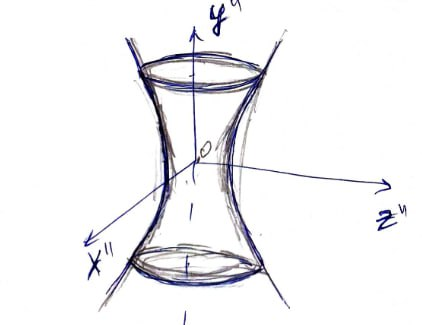
\includegraphics[width=10cm]{source/7.jpg}
\end{center}

\newpage

Итоговая замена координат выглядит следующим образом:
\[
    \begin{cases}
        x = -\d{1}{\sqrt{5}}y'' + \d{2}{\sqrt{5}}z'' \\
        y = x'' + 2                                  \\
        z = \d{2}{\sqrt{5}}y'' + \d{1}{\sqrt{5}}z''
    \end{cases}
\]

\answer{7}
\begin{itemize}
    \item Канонический вид: $2{x''}^2 - 4{y''}^2 + {z''}^2 = 3$;
    \item Поверхность: однополостный гиперболоид;
    \item Эскиз: выполнен сверху.
\end{itemize}
